\documentclass[8pt]{beamer}
\usepackage{tikz}
\usepackage[utf8]{vietnam}
\usepackage{amsmath}
\usepackage{graphicx}
\usepackage{wrapfig}
\usepackage{mathrsfs}
\usepackage{hyperref}
\usetheme{Copenhagen}
\usecolortheme{beaver}
\setbeamertemplate{navigation symbols}{}
\setbeamertemplate{headline}{}
\title[Chương 3: Biến đổi Fourier] %optional
{Chương 3: Biến đổi Fourier}
\subtitle{Tín hiệu và hệ thống}
\author[Tín hiệu và hệ thống] % (optional)
{Tín Vũ}
\date[VLC 2021] % (optional)
{tinvu1309@gmail.com}
\begin{document}
\frame{\titlepage}
\begin{frame}{Mục lục}
\tableofcontents
\end{frame}
\begin{frame}{Giới thiệu playlist}
\section{Giới thiệu playlist}
	\begin{itemize}
		\item Mình là Tín Vũ, hiện tại đang là sinh viên học tại Trường Đại học Công nghệ, Đại học Quốc gia Hà Nội. Mình tạo playlist video này để hỗ trợ các bạn học môn Tín hiệu và hệ thống trong các trường đại học kĩ thuật theo hướng \alert{trực quan hóa} nhất có thể.
		\item Do đó, mục tiêu của mình khi thực hiện playlist này không chỉ giúp các bạn ôn thi được điểm cao mà còn \alert{hiểu sâu công thức để làm nền tảng cho các môn học sau}.
		\item Để đạt được hai mục tiêu trên, các bạn nên xem \textbf{toàn bộ} video của mình, còn nếu chỉ cần ôn thi cấp tốc và đạt điểm cao thì hãy \textbf{bỏ qua} các video "optional".
		\item Nội dung playlist này chủ yếu bám sát nội dung môn học Tín hiệu và hệ thống tại trường của mình; nếu các bạn học trường khác, hãy tham khảo kĩ đề cương hay đề thi của trường bạn để đối chiếu sao cho ôn tập đúng trọng tâm và hợp lý. 
		\item Môn học này bao gồm \textbf{6} chương, các chương đều liên quan rất chặt chẽ và logic với nhau nên hãy học cẩn thận ngay từ \alert{chương 0} để ôn thi cuối kì đỡ vất vả.
	\end{itemize}
\end{frame}
\begin{frame}{Tài liệu tham khảo}
\section{Tài liệu tham khảo}
\begin{itemize}
		\item Tài liệu tham khảo chính: Signals and Systems (2nd edition) Alan V. Oppenheim and Alan S. Willsky.
		\item Tài liệu tham khảo phụ: Bài tập của mình học khóa trước, đề thi các năm cũ,...
		\item Tài liệu tham khảo phụ: Nếu bạn là sinh viên trường mình và muốn học "tủ" nhiều bài thì nên đọc Signals and Systems (2nd edition) Simon Haykin vì các thầy cô chủ yếu dạy và ra đề trong cuốn này, thế nhưng mình đánh giá cuốn này không đầy đủ và chi tiết như sách của Alan V. Oppenheim. 
	\end{itemize}
\end{frame}
\begin{frame}{Giới thiệu về Fourier}
\section{Giới thiệu về Fourier}
\begin{wrapfigure}{l}{0.4\textwidth} %this figure will be at the right
    \centering
    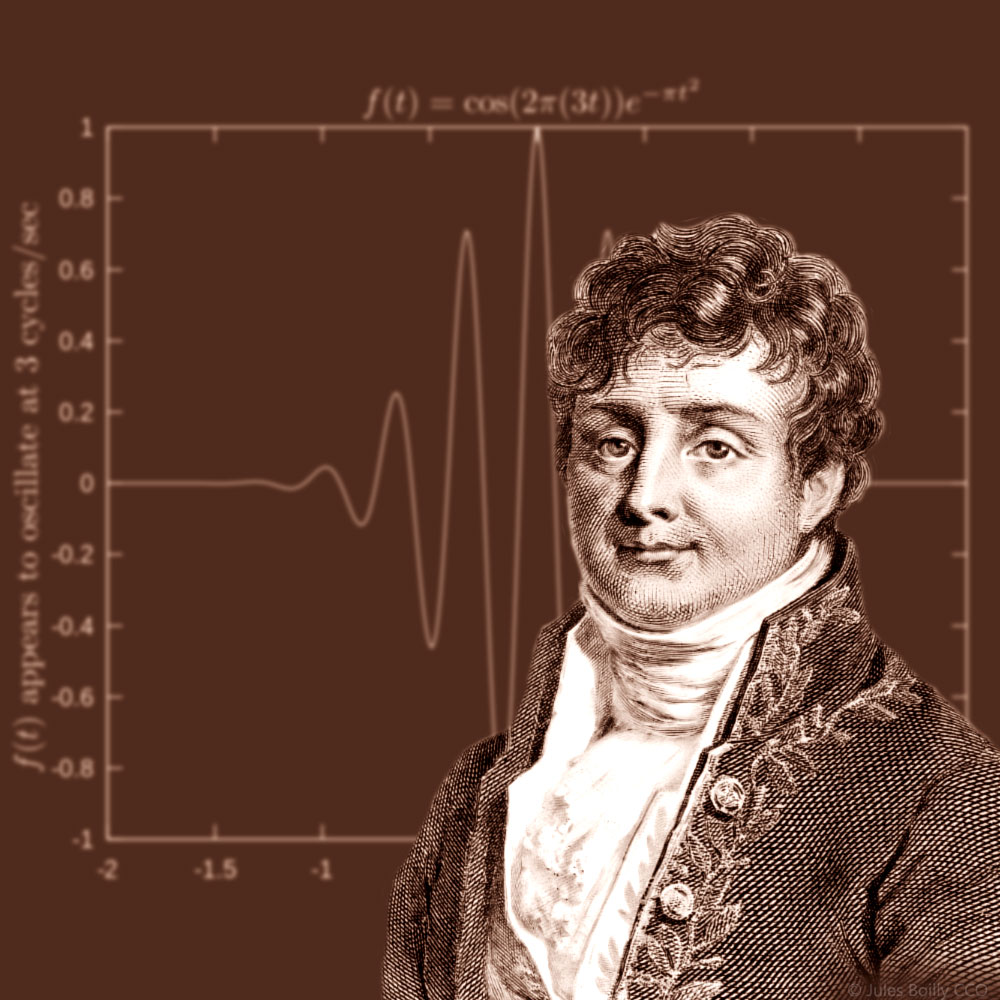
\includegraphics[width=0.4\textwidth]{Fourier-1000.jpg}
\end{wrapfigure}
Joseph Fourier là nhà toán học huyền thoại \\
người Pháp sống ở thế kỉ 18. Công trình nổi tiếng nhất của 
ông là phép biến đổi Fourier được ông nghiên cứu khi giải quyết bài toán \\
truyền nhiệt đã đặt nền móng cho toàn bộ lĩnh vực xử lý tín hiệu phát triển mạnh mẽ sau này. 
\\ Phép biến đổi Fourier chính là trái tim\\ của toàn bộ ngành khoa học kĩ thuật hiện đại.

\end{frame}
\begin{frame}{Giới thiệu về Fourier}
\begin{figure}[h]
			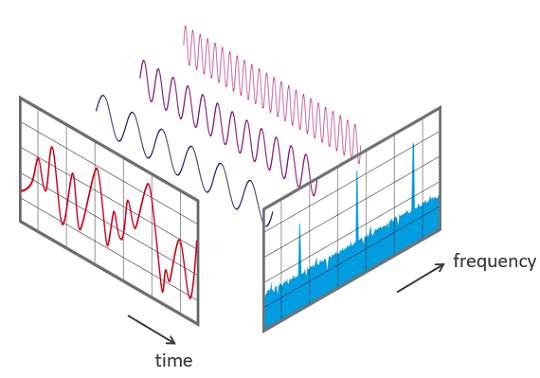
\includegraphics[width=0.9\textwidth]{FFT-Time-Frequency-View-540.png}
			\caption{Fourier Transform Visualization}\label{fig:re11}
		\end{figure}

\end{frame}
\begin{frame}{Chuỗi Fourier (FS)}
	\section{Chuỗi Fourier (FS)}
\subsection{Chuỗi Fourier liên tục (CTFS)}
\begin{itemize}
	\item Chuỗi Fourier liên tục (CTFS)
\end{itemize}
\subsubsection{Khái niệm chuỗi Fourier liên tục}
\begin{itemize}
	\item[-] Khái niệm chuỗi Fourier liên tục
\end{itemize}
Một tín hiệu $x(t)$ \alert{liên tục} và \textbf{tuần hoàn} bất kì đều có thể được biểu diễn dưới dạng tổng của các tín hiệu tuần hoàn khác:
$$x(t)=\sum_{k=-\infty}^{+\infty}a_{k}e^{jk\omega_{0} t}=\sum_{k=-\infty}^{+\infty}a_{k}e^{jk\frac{2\pi}{T_{0}}t}$$
Hệ số $a_{k}$ được tìm ra như sau, với $n$ là số nguyên tùy ý:
\begin{equation*}
\begin{split}
	x(t)e^{-jn\omega_{0}t}&=\sum_{k=-\infty}^{+\infty}a_{k}e^{jk\omega_{0}t}e^{-jn\omega_{0}t}
	\\ \Leftrightarrow \int_{T_{0}}x(t)e^{-jn\omega_{0}t}dt&=\int_{T_{0}}\sum_{k=-\infty}^{+\infty}a_{k}e^{jk\omega_{0}t}e^{-jn\omega_{0}t}dt\\
							       &=\sum_{k=-\infty}^{+\infty}a_{k}\left[\int_{T_{0}}e^{j(k-n)\omega_{0}t}dt\right]
\end{split}
\end{equation*}
Với $n\neq k$, hiển nhiên tích phân bằng $0$ (do bản chất tích phân của hàm tuần hoàn trên một chu kì), vậy khi và chỉ khi $n=k$ thì tích phân mới có giá trị xác định bằng $T_{0}$.
\end{frame}
\begin{frame}{Chuỗi Fourier (FS)}

\\ Vậy ta thu được công thức tính hệ số chuỗi FS liên tục (CTFS):
$$\alert{a_{k}=\frac{1}{T_{0}}\int_{T_{0}}x(t)e^{-jk\omega_{0}t}dt}$$
Khi giải bài tập, với tín hiệu đơn giản ta khai triển trực tiếp bằng cách tách tín hiệu gốc thành dạng mũ phức, còn với tín hiệu phức tạp ta sử dụng công thức trên để tìm hệ số FS.
\\ Ví dụ 1: khai triển tín hiệu sau thành chuỗi Fourier liên tục:
$$x(t)=\cos(\omega_{0}t)$$
Ta rất dễ dàng khai triển tín hiệu trên theo công thức Euler từ định nghĩa:
$$x(t)=\frac{1}{2}\left(e^{j\omega_{0}t}+e^{-j\omega_{0}t}\right)=\frac{1}{2}e^{j\omega_{0}t}+\frac{1}{2}e^{-j\omega_{0}t}$$
Ta tìm được các hệ số chuỗi Fourier như sau:
\begin{equation*}
	a_{k}=
	\begin{cases}
		\frac{1}{2}\; (k=-1\; , k=1)	\\
		0 \;(\text{otherwise})\\
\end{cases}
\end{equation*}
Vậy ta kết luận: tín hiệu $x(t)$ được cấu tạo từ hai tín hiệu tuần hoàn nhỏ hơn, với cả hai tín hiệu thành phần đều có \alert{biên độ} bằng $\frac{1}{2}$, \alert{tần số góc} bằng $\omega_{0}$ , $-\omega_{0}$ và \alert{pha ban đầu} đều bằng $0$ rad. \\$\Rightarrow$ \textbf{Tại sao lại xuất hiện thành phần tần số góc âm ?}
\end{frame}
\begin{frame}{Chuỗi Fourier (FS)}
\begin{figure}[h]
			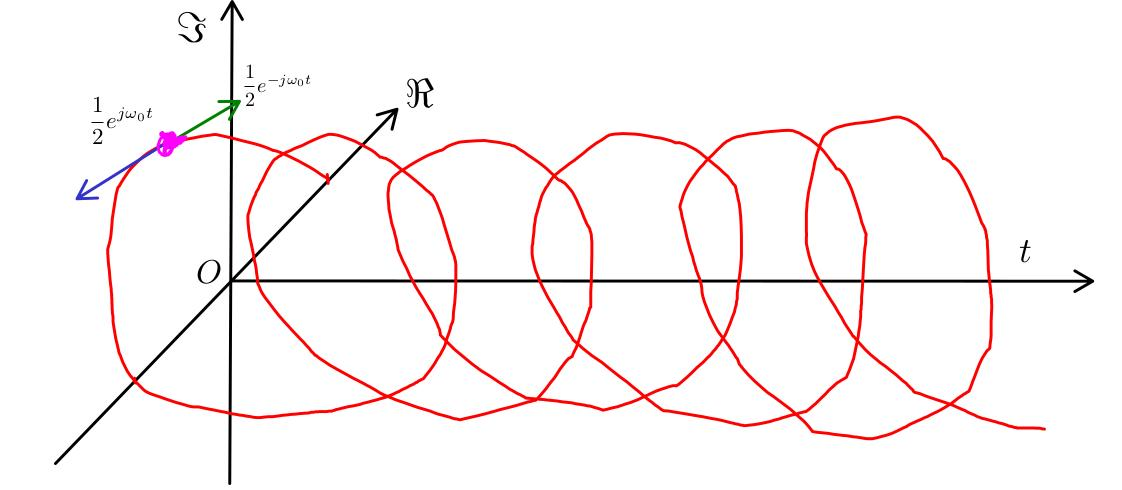
\includegraphics[width=0.5\textwidth]{helix.jpg}
			\caption{Harmonic component helix curve}\label{fig:re11}
		\end{figure}
\begin{figure}[h]
			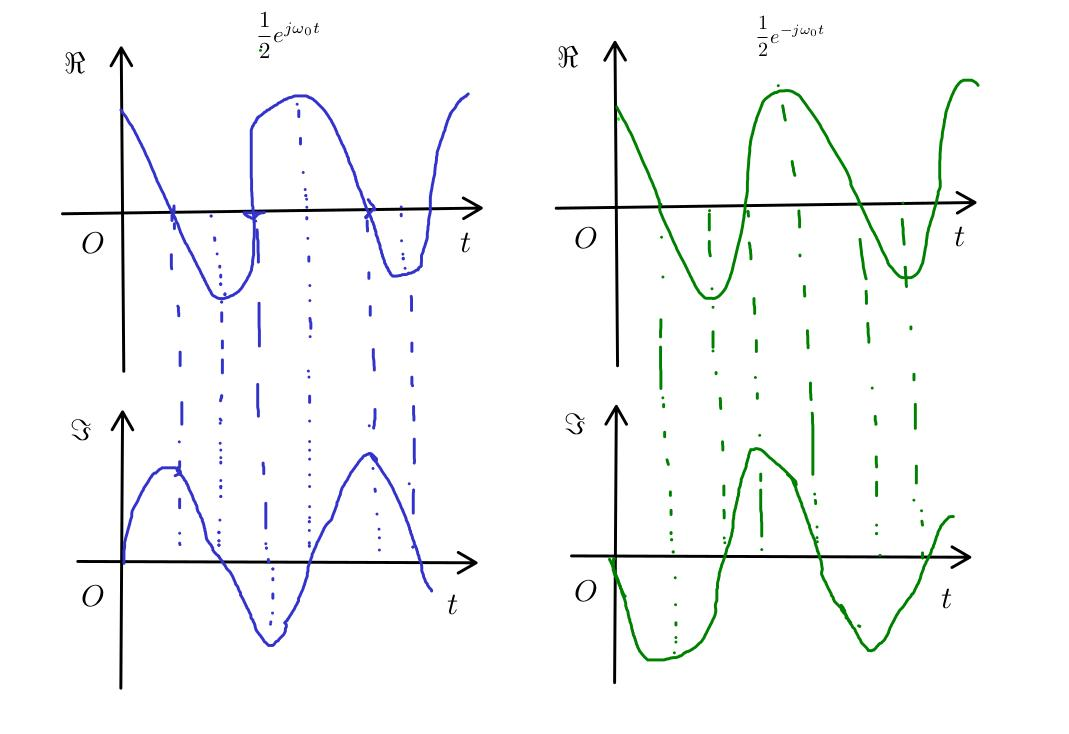
\includegraphics[width=0.5\textwidth]{imaginary.jpg}
			\caption{Negative Frequency Explaination}\label{fig:re11}

		\end{figure}
\end{frame}
\begin{frame}{Chuỗi Fourier (FS)}
\begin{figure}[h]
			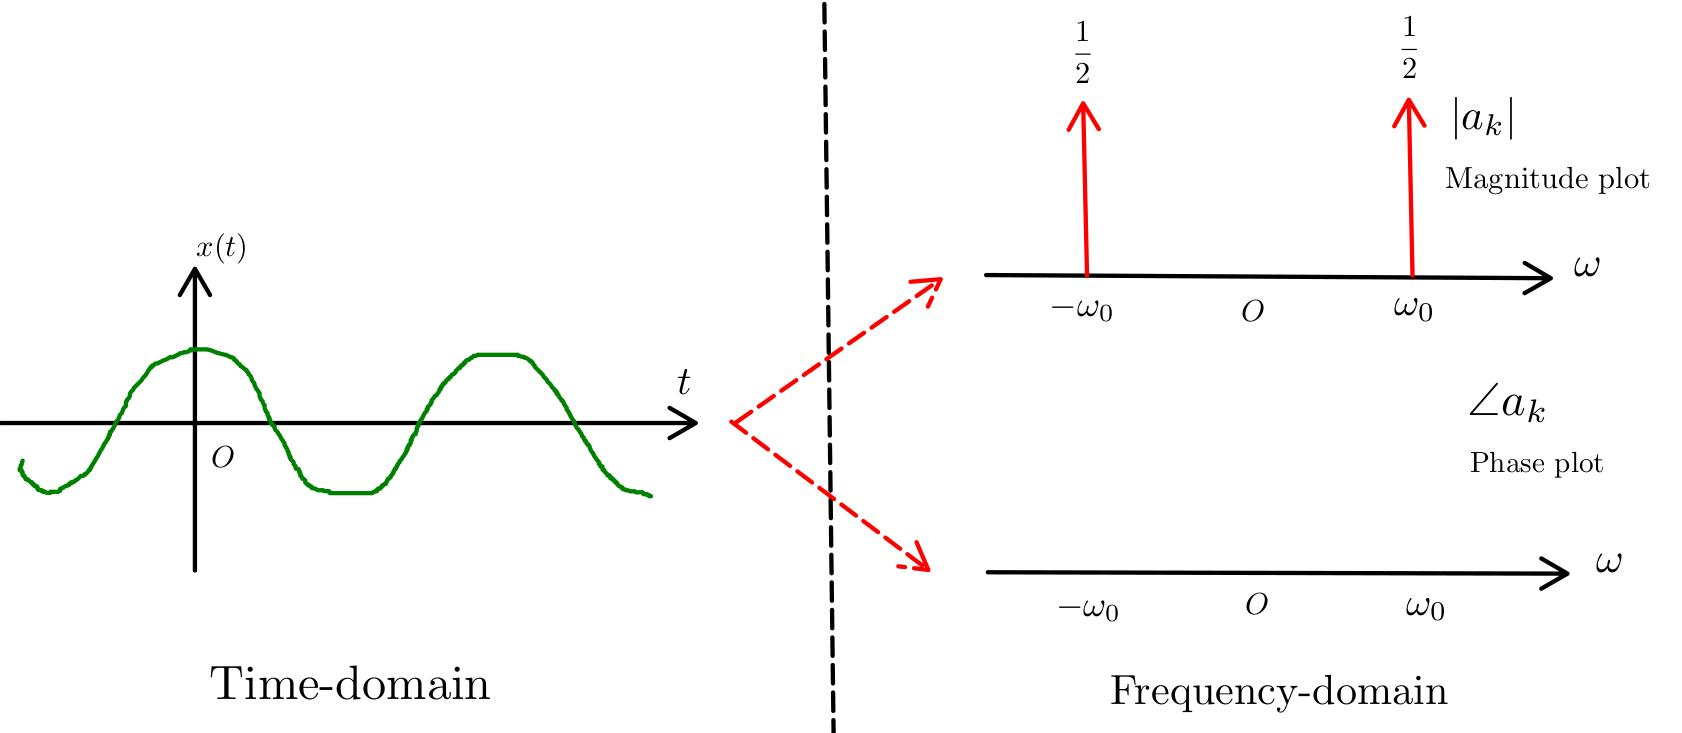
\includegraphics[width=0.47\textwidth]{fre.jpg}
			\caption{Simple cosine signal spectrum}\label{fig:re11}

		\end{figure}

		Suy ngẫm: vẽ phổ tín hiệu sine, giải thích nguyên nhân xuất hiện thành phần \textbf{tần số âm}. Nếu loại bỏ thành phần \textbf{tần số âm} thì sao? 
$$x(t)=\sin{(\omega_{0}t)}$$
\begin{figure}[h]
			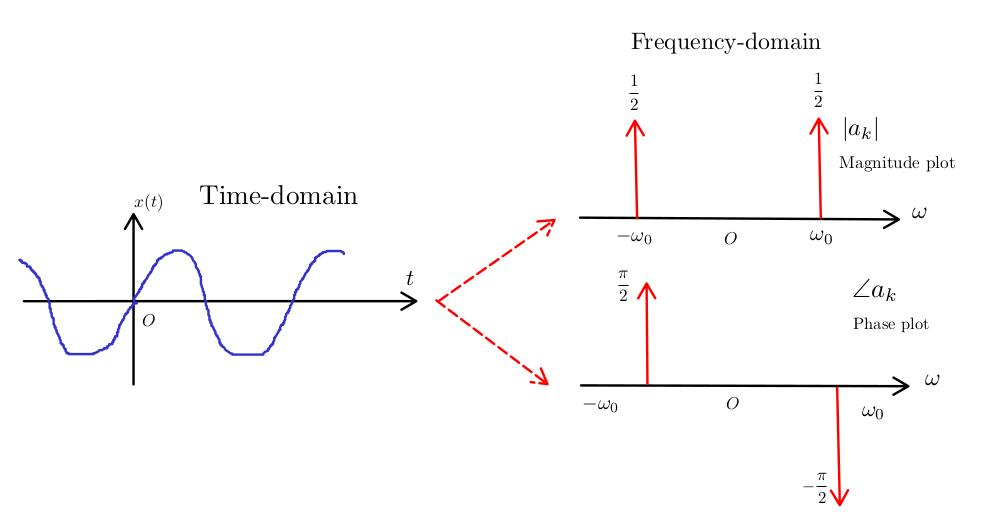
\includegraphics[width=0.47\textwidth]{sine.jpg}
			\caption{Simple sine signal spectrum}\label{fig:re11}

		\end{figure}


\end{frame}
\begin{frame}{Chuỗi Fourier (FS)}
Ví dụ 2: khai triển tín hiệu sau thành chuỗi Fourier liên tục:
\begin{figure}[h]
			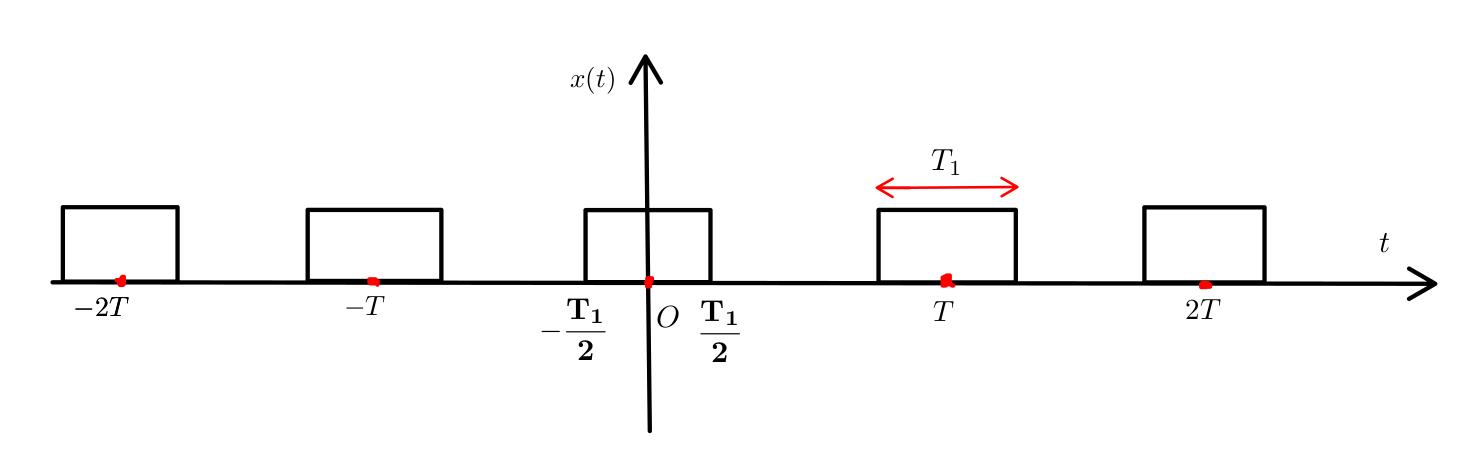
\includegraphics[width=0.6\textwidth]{square.jpg}
			\caption{Square wave signal in time-domain}\label{fig:re11}

		\end{figure}
		Để khai triển tín hiệu trên thành chuỗi Fourier liên tục, ta phải dùng công thức tính $a_{k}$ chứ không thể tách trực tiếp được nữa:
\begin{equation*}
\begin{split}
a_{k}=\frac{1}{T}\int_{T}x(t)e^{-jk\omega_{0}t}dt
\end{split}
\end{equation*}
Xét trường hợp đặc biệt $k=0$, ta có: $$a_{0}=\frac{1}{T}\int_{T}dt=\frac{1}{T}\int_{-\frac{T_{1}}{2}}^{\frac{T_{1}}{2}}dt=\frac{T_{1}}{T}$$
Với $k\neq 0$, ta có:
\begin{equation*}
	\begin{split}
		a_{k}=\frac{1}{T}\int_{T}x(t)e^{-jk\omega_{0}t}dt=\frac{1}{T}\int_{-\frac{T_{1}}{2}}^{\frac{T_{1}}{2}}e^{-jk\omega_{0}t}dt=\frac{\sin{\left(k\omega_{0}\frac{T_{1}}{2}\right)}}{k\pi}
\end{split}
\end{equation*}
\end{frame}
\begin{frame}{Chuỗi Fourier (FS)}
Vậy ta thu được hệ số chuỗi Fourier liên tục:
\begin{equation*}
	a_{k}=
	\begin{cases}
		\frac{T_{1}}{T} \; (k=0)\\
		\frac{\sin{\left(k\omega_{0}\frac{T_{1}}{2}\right)}}{k\pi} \;(k\neq0)\\

	\end{cases}
\end{equation*}
\begin{figure}[h]
			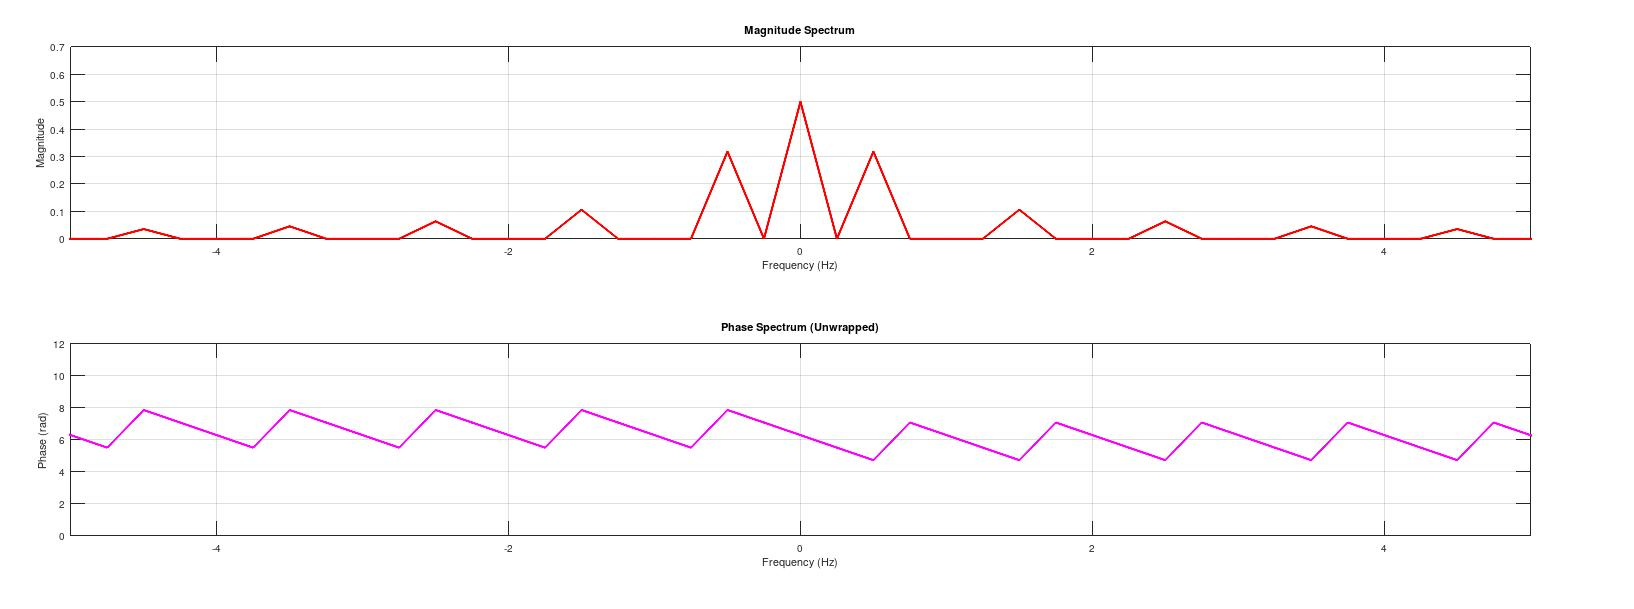
\includegraphics[width=0.9\textwidth]{s.jpg}
			\caption{Square wave signal in frequency-domain}\label{fig:re11}

		\end{figure}
	Suy ngẫm: các bạn hãy thử tự giải lại ví dụ 1 bằng công thức tính $a_{k}$ như ở trên.
\end{frame}
\begin{frame}{Chuỗi Fourier (FS)}
\subsubsection{Tính chất chuỗi Fourier liên tục}
\begin{itemize}
	\item[-] Tính chất chuỗi Fourier liên tục
\end{itemize}
\begin{block}{Continuous-time Fourier  Series Pair}
\begin{equation*}
\begin{split}
	x(t)&=\sum_{k=-\infty}^{+\infty}a_{k}e^{jk\omega_{0}t}\\
	a_{k}&=\frac{1}{T_{0}}\int_{T_{0}}x(t)e^{-jk\omega_{0}t}dt\\
\end{split}
\end{equation*}
\end{block}
Ta định nghĩa phép toán biến đổi chuỗi tín hiệu liên tục $x(t)$ về chuỗi Fourier liên tục như sau:
$$\mathscr{FS}(x(t))=a_{k}$$
Xét cặp tín hiệu $x(t)$ và $y(t)$ tương ứng có phép toán biến đổi chuỗi Fourier liên tục tương ứng:
$$\mathscr{FS}(x(t))=a_{k}$$
$$\mathscr{FS}(y(t))=b_{k}$$
Ta xét các tính chất cơ bản của chuỗi Fourier liên tục như sau:
\end{frame}
\begin{frame}{Chuỗi Fourier (FS)}
\begin{enumerate}
	\item[1] Tính tuyến tính:
\begin{equation*}
\begin{split}
	\mathscr{FS}(\alpha x(t)+\beta y(t))&=\frac{1}{T_{0}}\int_{T_{0}}(\alpha x(t)+\beta y(t))e^{-jk\omega_{0}t}dt\\
					    &= \alpha\frac{1}{T_{0}}\int_{T_{0}}x(t)e^{-jk\omega_{0}t}dt+\beta\frac{1}{T_{0}}\int_{T_{0}}y(t)e^{-jk\omega_{0}t}dt\\
					    &= \alpha\mathscr{FS}(x(t))+\beta\mathscr{FS}(y(t))
\end{split}
\end{equation*}
Như đã thảo luận ở \alert{chương 1}, ta có thể tổng quát hóa bài toán xét tính tuyến tính cho tổ hợp tuyến tính của vô số tín hiệu.
\item[2] Dịch thời gian:
\begin{equation*}
\begin{split}
	\mathscr{FS}(x(t-t_{0}))&=\frac{1}{T_{0}}\int_{T_{0}}x(t-t_{0})e^{-jk\omega_{0}t}dt\\
				&= \frac{1}{T_{0}}\int_{T_{0}}x(t-t_{0})e^{-jk\omega_{0}(t-t_{0})}e^{-jk\omega_{0}{t_{0}}}d(t-t_{0})\\
				&= e^{-jk\omega_{0}t_{0}}a_{k}
\end{split}
\end{equation*}
\end{enumerate}
\end{frame}
\begin{frame}{Chuỗi Fourier (FS)}
\begin{enumerate}
	\item[3] Lật tín hiệu:
\begin{equation*}
\begin{split}
	\mathscr{FS}(x(-t))&=\frac{1}{T_{0}}\int_{T_{0}}x(-t)e^{-jk\omega_{0}t}dt=\frac{-1}{T_{0}}\int_{T_{0}}x(-t)e^{-jk\omega_{0}t}d(-t)\\
			   &= \frac{1}{T_{0}}\int_{T_{0}}x(t)e^{jk\omega_{0}t}dt=a_{-k}
\end{split}
\end{equation*}
\item[4] Co dãn trong miền thời gian:
$$\mathscr{FS}(x(\alpha t))=a_{k}$$
do co dãn trong miền thời gian chỉ làm ảnh hưởng đến tần số $\omega_{0}\to \alpha\omega_{0}$ chứ không làm ảnh hưởng đến hệ số $a_{k}$.
\item[5] Phép vi phân:
\begin{equation*}
\begin{split}
\mathscr{FS}\left(\frac{dx(t)}{dt}\right)&=jk\omega_{0}a_{k}
\end{split}
\end{equation*}
\item [6] Phép tích phân:
	$$\mathscr{FS}\left(\int_{-\infty}^{t}x(\tau)d\tau\right)=\frac{a_{k}}{jk\omega_{0}}$$
\end{enumerate}
\end{frame}
\begin{frame}{Chuỗi Fourier (FS)}
	\begin{enumerate}
\item[7] Phép tích thường (tích điều chế):
\begin{equation*}
\begin{split}
	\mathscr{FS}(x(t)y(t))&=\frac{1}{T_{0}}\int_{T_{0}}(x(t)y(t))e^{-jk\omega_{0}t}dt\\&=\frac{1}{T_{0}}\int_{T_{0}}x(t)\left(\sum_{k=-\infty}^{+\infty}b_{k}e^{jn\omega_{0}t}\right)e^{-jk\omega_{0}t}dt\\&=\frac{1}{T_{0}}\sum_{k=-\infty}^{+\infty}b_{k}\int_{T_{0}}x(t)e^{j(n-k)\omega_{0}t}dt\\&=\sum_{k=-\infty}^{+\infty}b_{k}a_{n-k}=b_{k}*a_{k}
\end{split}
\end{equation*}
\item[8] Đẳng thức năng lượng Parseval: 
$$\frac{1}{T_{0}}\int_{T_{0}}|x(t)|^2dt=\sum_{k=-\infty}^{+\infty}|a_{k}|^2$$
Công suất trung bình của tín hiệu trong một chu kì (vế trái) bằng \textbf{tổng các hệ số chuỗi Fourier của tín hiệu} (vế phải). Đẳng thức này rất khó để có thể chứng minh đơn giản, nên ở đây ta chỉ có thể hiểu đại khái ý tưởng của nó như sau: xét một thành phần điều hòa có tần số góc bằng $k\omega_{0}$ ngẫu nhiên trong tín hiệu $x(t)$, hiến nhiên ta có công suất trung bình của nó trong một chu kì là:
	\end{enumerate}
\end{frame}
\begin{frame}{Chuỗi Fourier (FS)}
	\begin{enumerate}
		\item[]
	$$\frac{1}{T_{0}}\int_{T_{0}}|x_{k}(t)|^2dt=\frac{1}{T_{0}}\int_{T_{0}}|a_{k} e^{jk\omega_{0}t}|^2dt=|a_{k}|^2$$
	Vậy với một tín hiệu $x(t)$ gồm nhiều thành phần điều hòa, ta có:

$$\frac{1}{T_{0}}\int_{T_{0}}|x(t)|^2dt=\sum_{k=-\infty}^{+\infty}|a_{k}|^2$$
\end{enumerate}
Từ 8 tính chất cơ bản của chuỗi Fourier liên tục này, ta có thể giải bài tập nhanh hơn rất nhiều so với áp dụng trực tiếp cặp công thức CTFS pair đã đề cập ở trên. Tất nhiên, do đây không phải là phần nằm trọng tâm trong nội dung thi, nên chúng ta sẽ chỉ lướt rất nhanh qua một ví dụ đơn giản: 
sóng vuông $x(t)$ được biểu diễn như hình vẽ dưới đây có hệ số Fourier liên tục $a_{k}$, hãy xác định hệ số Fourier $b_{k}$ của tín hiệu $y(t)$.
\begin{figure}[h]
			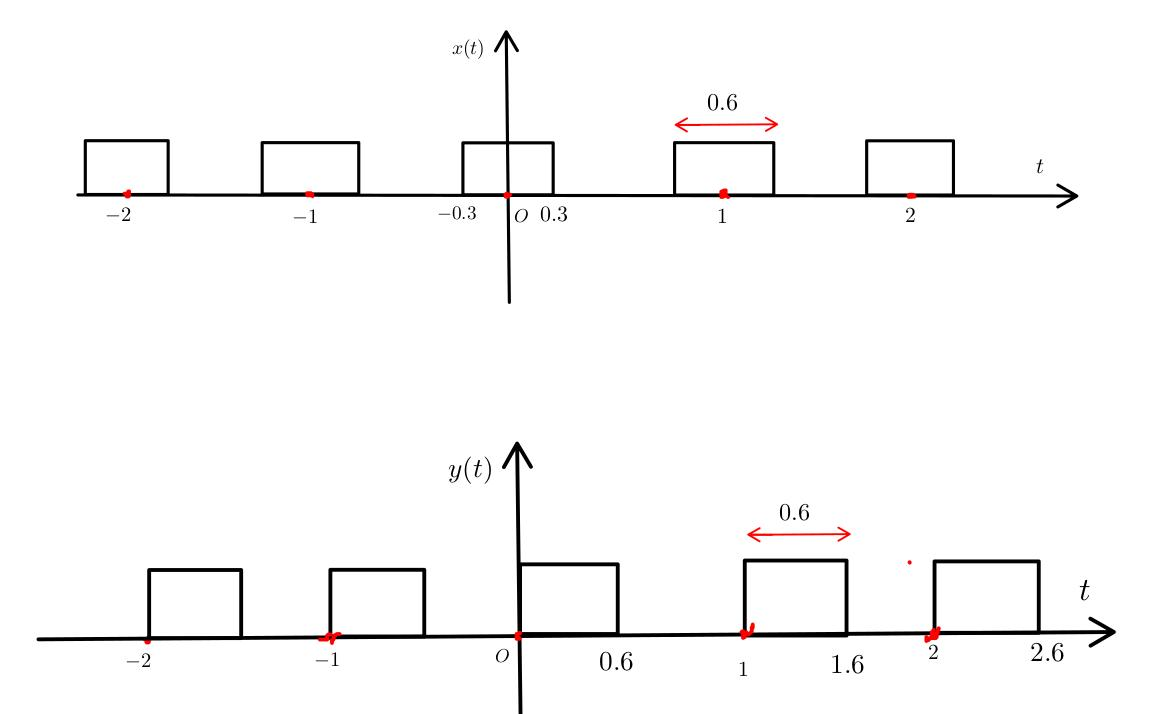
\includegraphics[width=0.46\textwidth]{pro.jpg}
			\caption{Square wave signal in time-domain}\label{fig:re11}

		\end{figure}

\end{frame}
\begin{frame}{Chuỗi Fourier (FS)}
Ta dễ thấy:
$$y(t)=x(t-0.3)\Rightarrow \mathscr{FS}(y(t))=\mathscr{FS}(x(t-0.3))=a_{k}e^{-jk\frac{2\pi}{T_{0}}0.3}=a_{k}e^{-jk0.6\pi}$$
Suy ngẫm: từ ví dụ 2 ở mục trước, các bạn hãy tính ra kết quả cuối cùng của bài toán này với gợi ý trên
\subsubsection{Đáp ứng của hệ thống LTI với tín hiệu tuần hoàn}
\begin{itemize}
	\item[-] Đáp ứng của hệ thống LTI với tín hiệu tuần hoàn
\end{itemize}
Trong \alert{Chương 2}, chúng ta đã xét một họ bài toán tìm đầu ra của hệ thống LTI với đầu vào cho trước bằng phép tích chập; ở đây ta xét một kết quả cực kì đặc biệt đặc trưng cho đầu ra của hệ thống với đầu vào là tín hiệu \textbf{tuần hoàn}. 
\begin{figure}[h]
			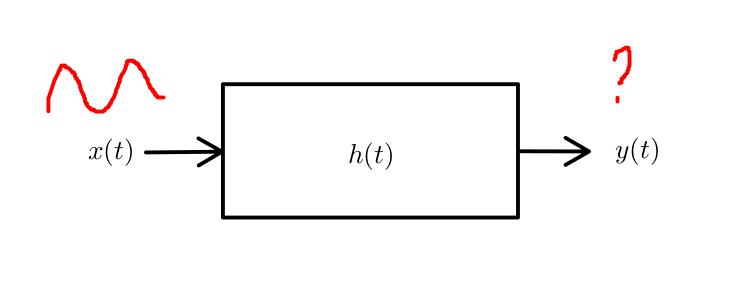
\includegraphics[width=0.46\textwidth]{ht.jpg}
			\caption{If the input of LTI system is periodic signal, what's the output ?}\label{fig:re11}

		\end{figure}
Vì $x(t)$ là tín hiệu \textbf{tuần hoàn}, nên ta có thể tách $x(t)$ thành chuỗi Fourier liên tục:
$$x(t)=\sum_{k=-\infty}^{+\infty}a_{k}e^{jk\omega_{0} t}$$
\end{frame}
\begin{frame}{Chuỗi Fourier (FS)}
Do tích chập có tính \alert{tuyến tính} nên ta có:
$$y(t)=x(t)*h(t)=\sum_{k=-\infty}^{+\infty}[(a_{k}e^{jk\omega_{0}t})*h(t)]=\sum_{k=-\infty}^{+\infty}x_{k}(t)*h(t)$$
Với $x_{k}(t)=a_{k}e^{jk\omega_{0}t}$ là một thành phần điều hòa của tín hiệu $x(t)$ lớn. Ta xét tích chập:
\begin{equation*}
\begin{split}
	y_{k}(t)=x_{k}(t)*h(t)&=\int_{-\infty}^{+\infty}x_{k}(\tau)h(t-\tau)d\tau=\int_{-\infty}^{+\infty}x_{k}(t-\tau)h(\tau)d\tau\\&=\int_{-\infty}^{+\infty}a_{k}e^{jk\omega(t-\tau)}h(\tau)d\tau=\int_{-\infty}^{+\infty}a_{k}e^{jk\omega t}h(\tau)e^{-jk\omega\tau}d\tau\\&=x_{k}(t)\int_{-\infty}^{+\infty}h(\tau)e^{-jk\omega\tau}d\tau
\end{split}
\end{equation*}
Ta kí hiệu:
$$H(j\omega)=\int_{-\infty}^{+\infty}h(\tau)e^{-jk\omega\tau}d\tau$$
là hàm số theo biến tần số $\omega$, và gọi hàm số này là \alert{đáp ứng tần số của hệ thống},
ta tiếp tục suy ra:
$$y(t)=\sum_{k=-\infty}^{+\infty}y_{k}(t)=\sum_{k=-\infty}^{+\infty}x_{k}(t)H(j\omega)$$
\end{frame}
\end{document}
